



\section{Experimental Setup} %TODO
Even though the focus of this thesis lies in theoretical research, we consider it important to at least roughly analyze the practical \enquote{real world} efficiency of ever yalgorithm. All of them were implemented and tested on a set of deterministic parity automata.

The programming language of choice was C++14. The source code can be found in \cite{Tollkoetter2018}. The computer used to run the tests was an Arch Linux 4.19.4 64 bit machine powered by an AMD Ryzen 5 1600 processor and 16 GB DDR4-2400 RAM.


Several automata generated randomly using different parameters were used in the testing process. Three major different techniques of generation were used:

\begin{enumerate}
	\item Use Spot (\cite{duret.16.atva2}) to generate a random DPA. (called \textsf{gendet})
	\item Use Spot to generate a random non-deterministic B\"uchi automaton and use Spot again to convert it to a DPA. (called \textsf{detspot})
	\item Use Spot to generate a random non-deterministic B\"uchi automaton and use nbautils (\cite{Pirogov2018}) to convert it to a DPA. (called \textsf{detnbaut})
\end{enumerate}

Figures \ref{fig:rawstats:rawstats_size}, \ref{fig:rawstats:rawstats_prios}, \ref{fig:rawstats:rawstats_sccs}, \ref{fig:rawstats:rawstats_langclasnum} and \ref{fig:rawstats:rawstats_avg_langclassize} present some information about the automata. Regarding the number of states we stopped the generation at about 100 states, as most algorithms become too slow at that point. For the detnbaut set, the path refinement procedure can be sped up which is why the upper limit is higher. We elaborate this point in the relevant section.

The number of priorities is rather small in general. For gendet, we intentionally limited the number to 4 to mimic real world behavior that can be found in the detnbautils set. In comparison to nbautils, Spot does not perform priority reduction on the determinization result which explains why the detspot automata use more priorities in general.

The number of SCCs is consistently small among all three sets. detspot and gendet contain a few examples of automata with up to 60 SCCs but these are extreme outliers. This low number of SCCs is important to consider, as multiple of the algorithms such as the skip merger perform better the less connected the automaton is.

Finally, the average size of equivalence classes $\mathfrak{C}(\equiv_L)$. Again, this is of relevance to some of the reduction algorithms such as LSF as only states which are language equivalent can be merged. We can observe that the gendet set almost entirely consists of trivial classes (i.e. classes of size 1) while detspot and detnbaut show more promise in that regard.

\vspace{5pt}

Besides the three classes of data sets that we described above, we also looked at special families of automata that are specifically designed to be difficult to minimize; see \cite{Michel1988}. Unfortunately, these automata proved to be too difficult for our procedures and almost no algorithm could achieve any reduction on an automaton of any size. Thus, we will not discuss these results in any more detail in the upcoming chapters.

\begin{figure}
	\centering
	\begin{minipage}{0.49\textwidth}
		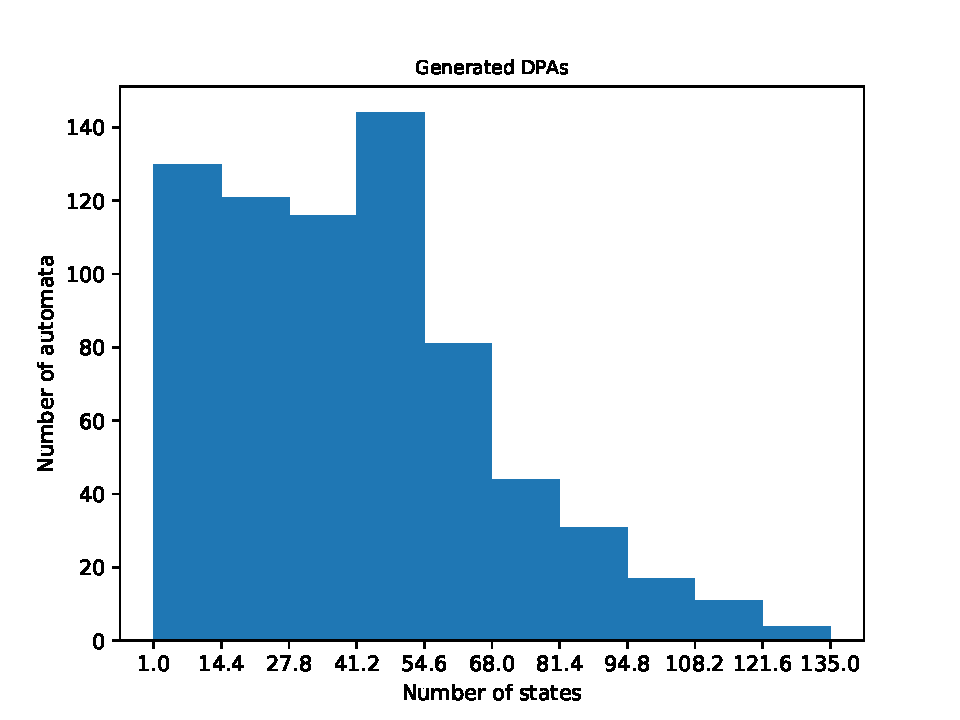
\includegraphics[page=1,height=.3\textheight]{../data/analysis/rawstats_gendet.pdf} 
		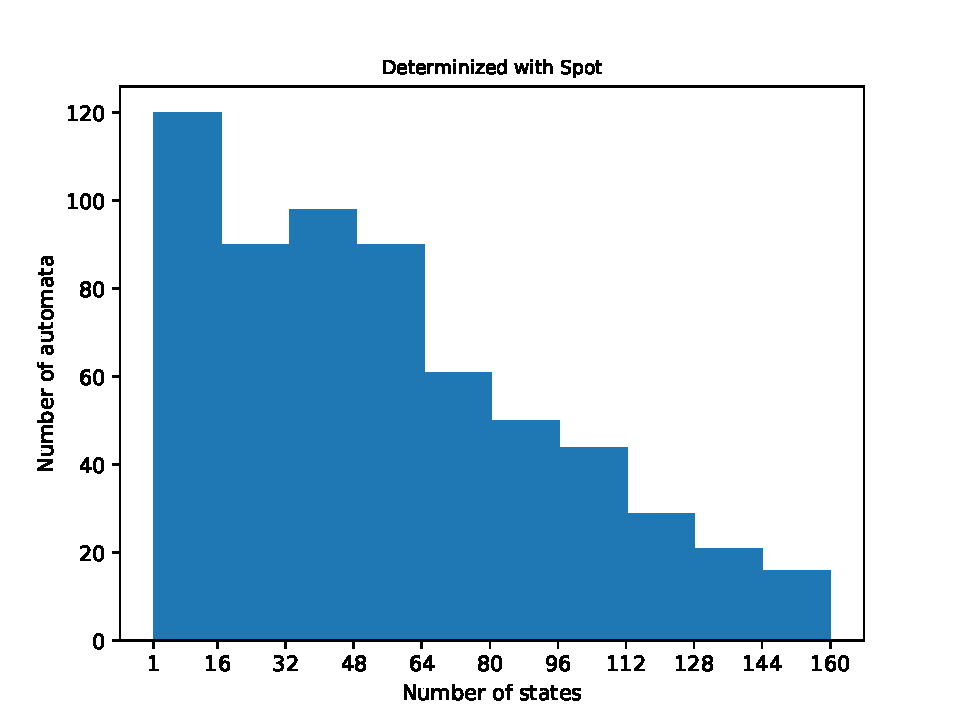
\includegraphics[page=1,height=.3\textheight]{../data/analysis/rawstats_detspot.pdf} 
		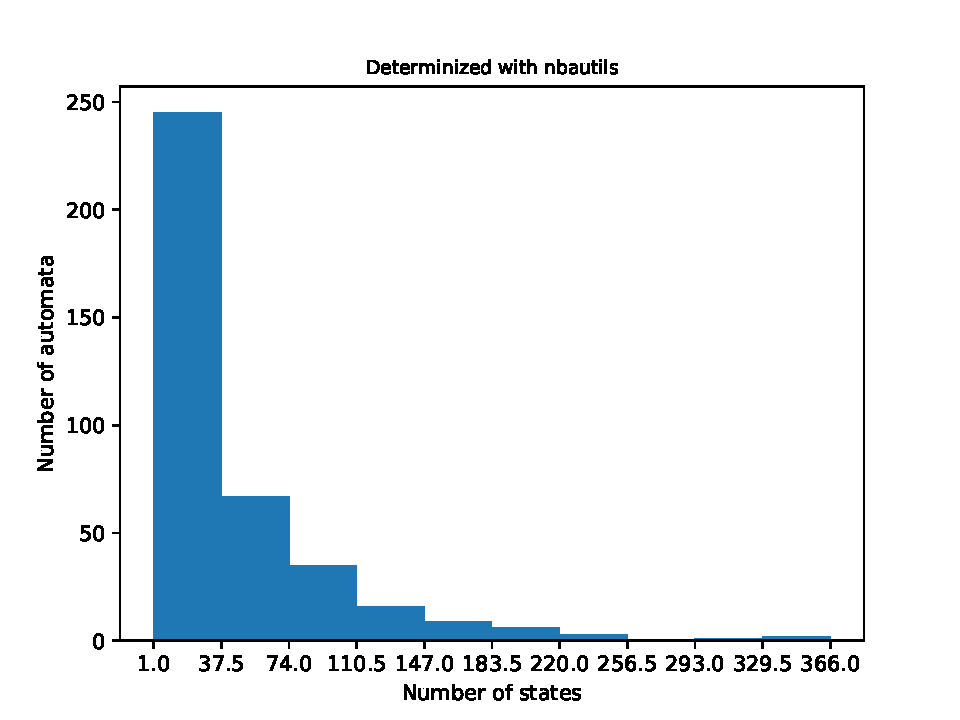
\includegraphics[page=1,height=.3\textheight]{../data/analysis/rawstats_detnbaut.pdf}
		\caption{Sizes of the automata in the testing environment.}
		\label{fig:rawstats:rawstats_size}
	\end{minipage}
	\hfill
	\begin{minipage}{0.49\textwidth}
		\includegraphics[page=2,height=.3\textheight]{../data/analysis/rawstats_gendet.pdf} 
		\includegraphics[page=2,height=.3\textheight]{../data/analysis/rawstats_detspot.pdf} 
		\includegraphics[page=2,height=.3\textheight]{../data/analysis/rawstats_detnbaut.pdf}
		\caption{Number of priorities in the automata in the testing environment.}
		\label{fig:rawstats:rawstats_prios}
	\end{minipage}
\end{figure}

\begin{figure}
	\centering
	\begin{minipage}{0.49\textwidth}
		\includegraphics[page=3,height=.3\textheight]{../data/analysis/rawstats_gendet.pdf} 
		\includegraphics[page=3,height=.3\textheight]{../data/analysis/rawstats_detspot.pdf} 
		\includegraphics[page=3,height=.3\textheight]{../data/analysis/rawstats_detnbaut.pdf}
		\caption{Number of SCCS in the automata in the testing environment.}
		\label{fig:rawstats:rawstats_sccs}
	\end{minipage}
	\hfill
	\begin{minipage}{0.49\textwidth}
		\includegraphics[page=4,height=.3\textheight]{../data/analysis/rawstats_gendet.pdf} 
		\includegraphics[page=4,height=.3\textheight]{../data/analysis/rawstats_detspot.pdf} 
		\includegraphics[page=4,height=.3\textheight]{../data/analysis/rawstats_detnbaut.pdf}
		\caption{Number of classes in $\mathfrak{C}(\equiv_L)$ that contain more than one state.}
		\label{fig:rawstats:rawstats_langclasnum}
	\end{minipage}
\end{figure}


\begin{figure}
	\centering
	\begin{minipage}{0.49\textwidth}
		\includegraphics[page=5,height=.3\textheight]{../data/analysis/rawstats_gendet.pdf} 
		\includegraphics[page=5,height=.3\textheight]{../data/analysis/rawstats_detspot.pdf} 
		\includegraphics[page=5,height=.3\textheight]{../data/analysis/rawstats_detnbaut.pdf}
		\caption{Average size of $\equiv_L$-classes of the automata in the testing environment.}
		\label{fig:rawstats:rawstats_avg_langclassize}
	\end{minipage}
\end{figure}


